% ........................................................................... %

This chapter presents the implementation of the contributions contained in this thesis work. We first present \emph{ServiceMosaic}, the umbrella project in which this work has been made. We then focus on the components that we have implemented for modeling and analyzing timed business protocols.

% ........................................................................... %

\section{ServiceMosaic}

% ........................................................................... %

This section presents the ServiceMosaic project. We first give an outlook of the general project architecture, then provide some technical details regarding how the various projects that compose ServiceMosaic are made.

% ........................................................................... %

\subsection{Project overview}

% ........................................................................... %

ServiceMosaic\footnote{See \url{http://servicemosaic.isima.fr/}} is an international project for research in the context of web services. It currently acts as a bridge between several research groups:
\begin{itemize}

	\item the SOC Group at the University of New South Wales, Sydney, Australia
	
	\item the APIS Research Group at Universit\'e Blaise Pascal, Clermont-Ferrand, France
	
	\item the BD-RCR Group at Universit\'e Claude Bernard, Lyon, France
	
	\item the group of Fabio Casati at the University of Trento, Italy.

\end{itemize}

\begin{figure}[tbhp]
    \centering
    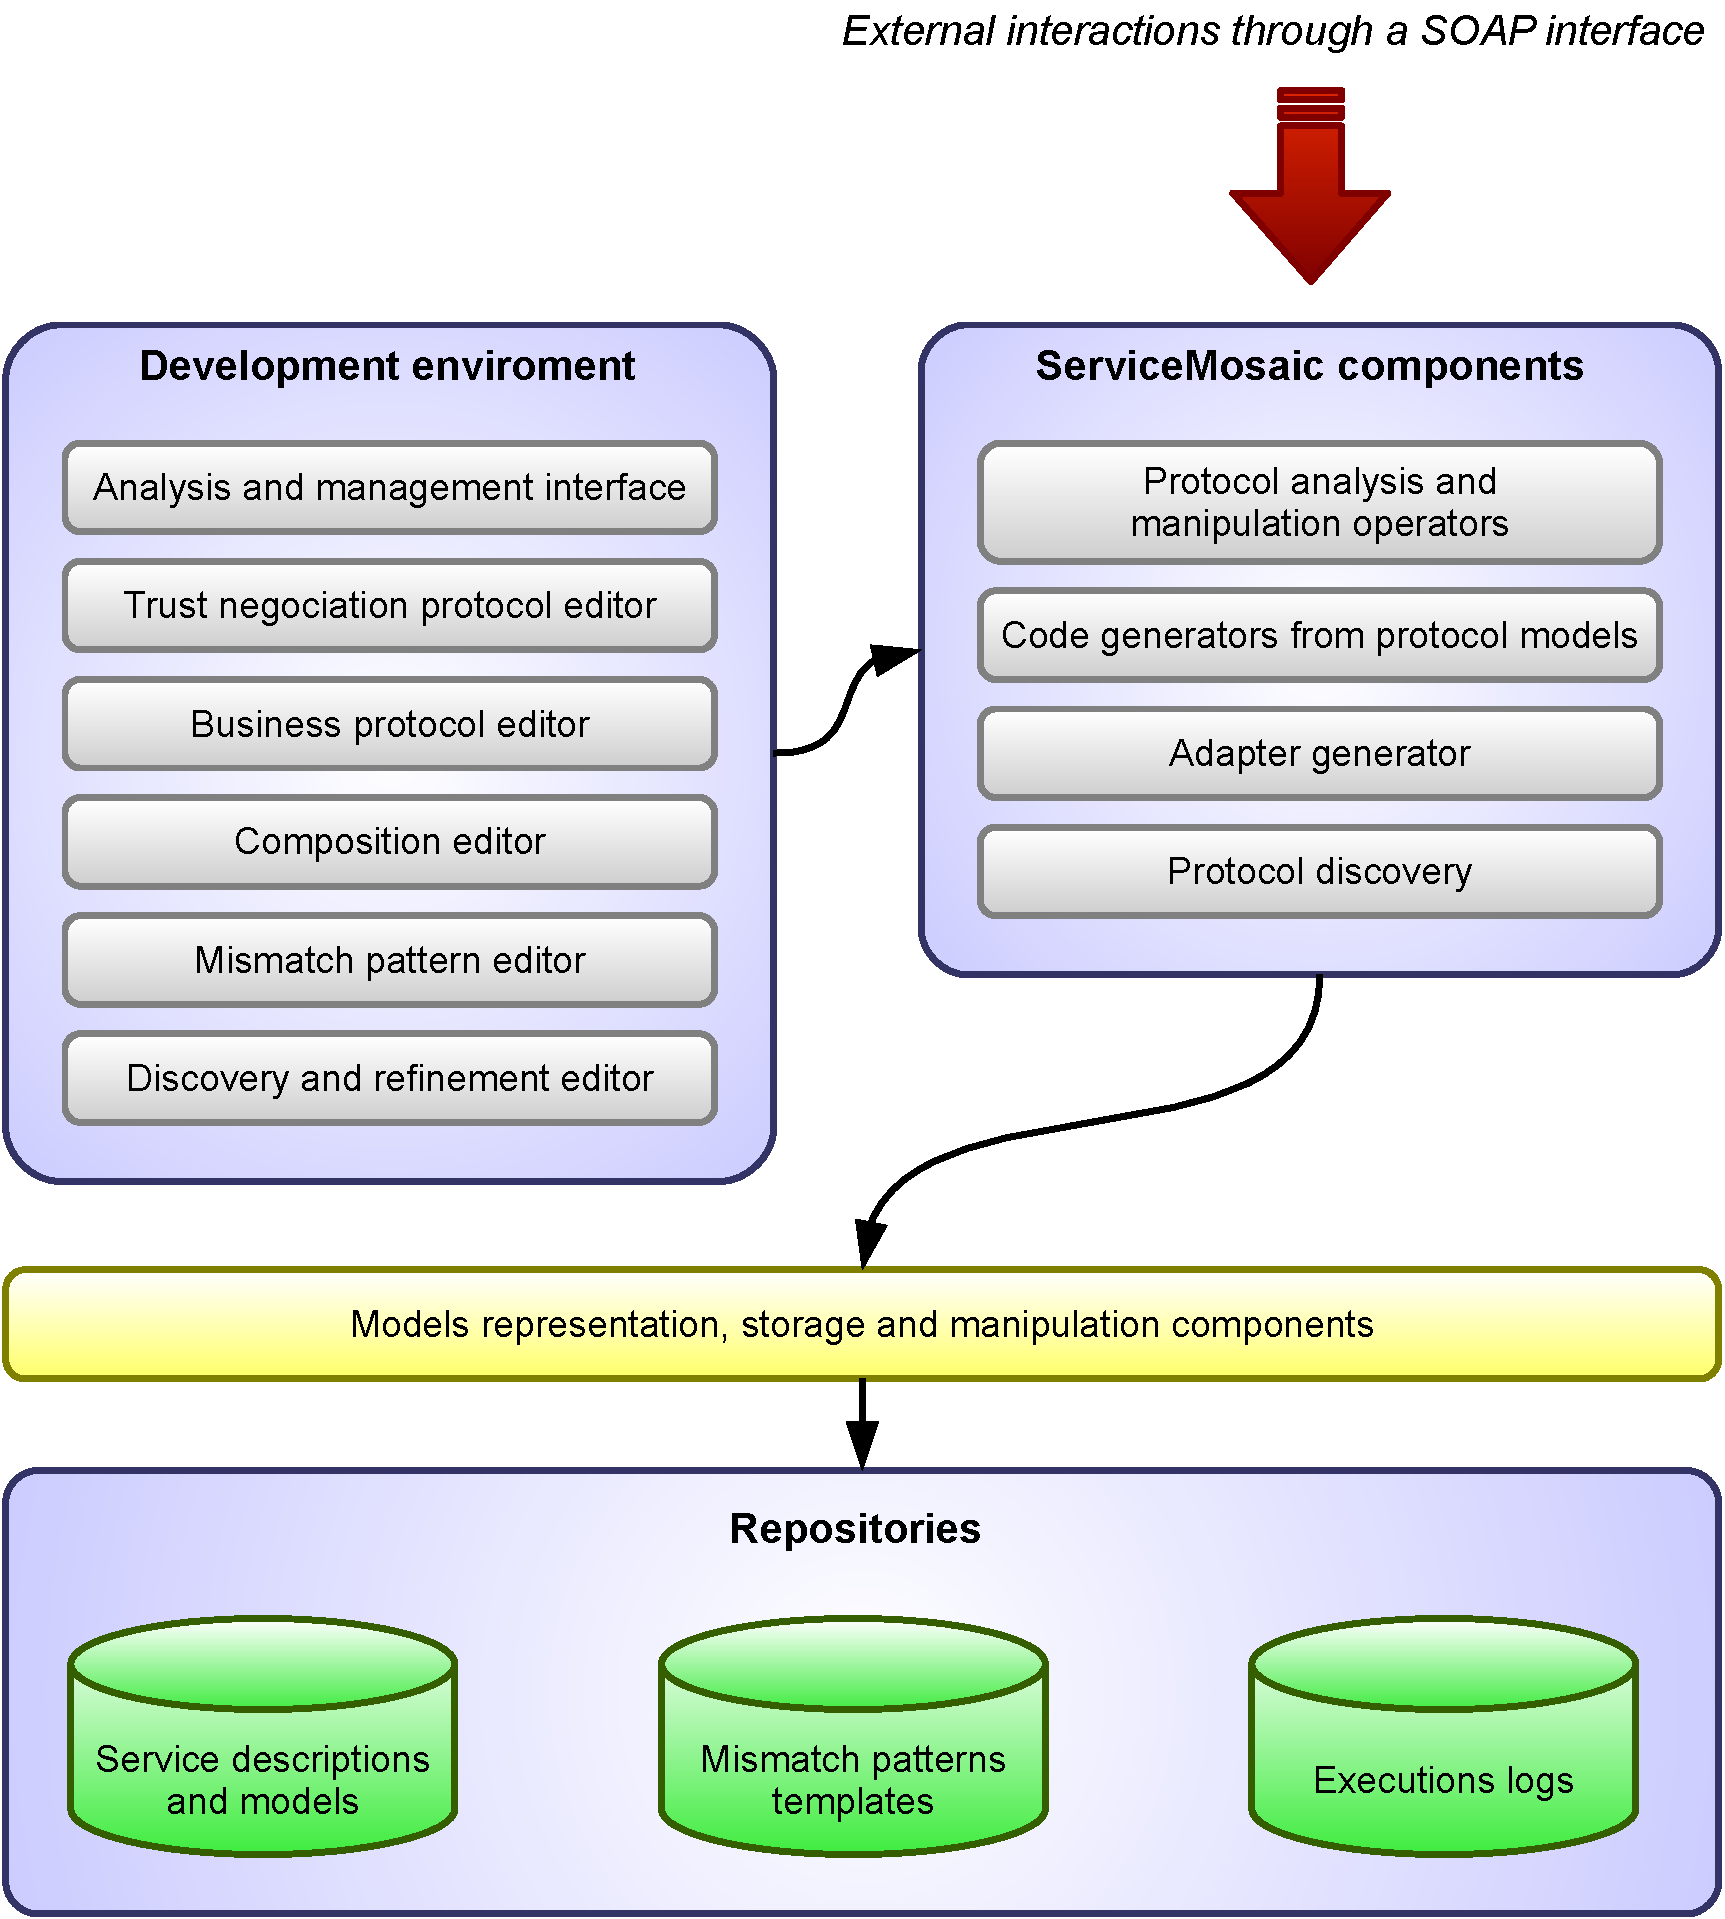
\includegraphics[width=\textwidth]{content/protocols-project/servicemosaic-architecture}
    \caption{Architecture overview of the ServiceMosaic platform.}
    \label{fig:servicemosaic-architecture}
\end{figure}

ServiceMosaic is a CASE platform for supporting the service development life-cycle that includes facilities for modeling, analyzing, discovering and adapting web service models \cite{BCTPM06-SM,NezhadSBCPT07}. The architecture, depicted on Figure~\ref{fig:servicemosaic-architecture}, comprises the following components.
\begin{description}
  
  \item[Models and manipulation components] support representing, storing an manipulating service descriptions and protocols. We provide basic manipulation operations of model elements such as protocols as core libraries that shield higher-level components from the details of their physical representations (e.g., plain files, XML, relational databases and so on).
  
  \item[Analysis and management components] include operators for protocol compatibility and replaceability analysis \cite{FTBB}, a code generator that produces BPEL skeletons from protocols \cite{BBFC04}, a code generator that produces BPEL templates for implementing the adapters \cite{BenatallahCGNT05,NezhadBMCC07}, and protocol discovery from service execution logs \cite{Motahari-NezhadSBC07}.
  
  \item[The development environment] provides visual exploration for modifying, analyzing and managing model elements. For example, it offers editors for business protocols, trust negotiation protocols \cite{SkogsrudBCD04,SkogsrudBC03} and orchestration models.
  
\end{description}

Finally, the ServiceMosaic components can be accessed through a set of programmatic SOAP web service interfaces. Each service is a simple thin wrapper on top of the components application programming interfaces.

% ........................................................................... %

\subsection{Technical overview}

% ........................................................................... %

The tools that we develop use the Java\tm platform version 5\footnote{See \url{http://java.sun.com/j2se/1.5.0/}}. Most developments are being made using the Java\tm programming language, but given the recent interest in dynamic languages that run on the Java\tm platform (e.g., Groovy, Ruby, Python, etc), we are allowing their use where useful. Indeed, the language facilities that are provided by some of those languages (e.g., functional programming inspired constructs such as closures\footnote{Martin Fowler gives a good concise presentation of closures at \url{http://martinfowler.com/bliki/Closure.html}}) allow for writing code that is arguably more concise and easier to read and maintain.\\

For every project, the development approach is the following:
\begin{enumerate}
  
  \item develop functionalities as standalone, reusable libraries that can be used in console, desktop, web or service-based tools, and
  
  \item expose the functionalities in development tools as plug-ins for the Eclipse platform\footnote{See \url{http://www.eclipse.org/}}.
  
\end{enumerate}

The choice of Eclipse as a development tools platform is justified by the following reasons. First of all, it is an open-source platform whose goal is to explicitly integrate tools from various vendors inside the same environment. As such, it provides several APIs and frameworks for building applications that can seamlessly integrate with third-party ones. The benefits for a research project are numerous.
\begin{enumerate}
  
  \item The implementation work can be focused on the sole contribution of each work, not on less critical details such as providing common dialog boxes, a preferences support framework, or integrated user assistance.
  
  \item The integration with new developments from inside the ServiceMosaic project or third-parties is vastly facilitated since a common foundation is being used. In most cases, the plug-ins that bring the contributions can simply be assembled inside an Eclipse-based environment without any modification having to be made.
  
  \item The Eclipse ecosystem is broad with a mixture of open-source and commercial offerings (see \url{http://www.eclipse.org/membership/exploreMembership.php}). As such, it is a positive factor for facilitating the dissemination of the work that we conduct.
  
\end{enumerate}

\begin{figure}[tbhp]
    \centering
    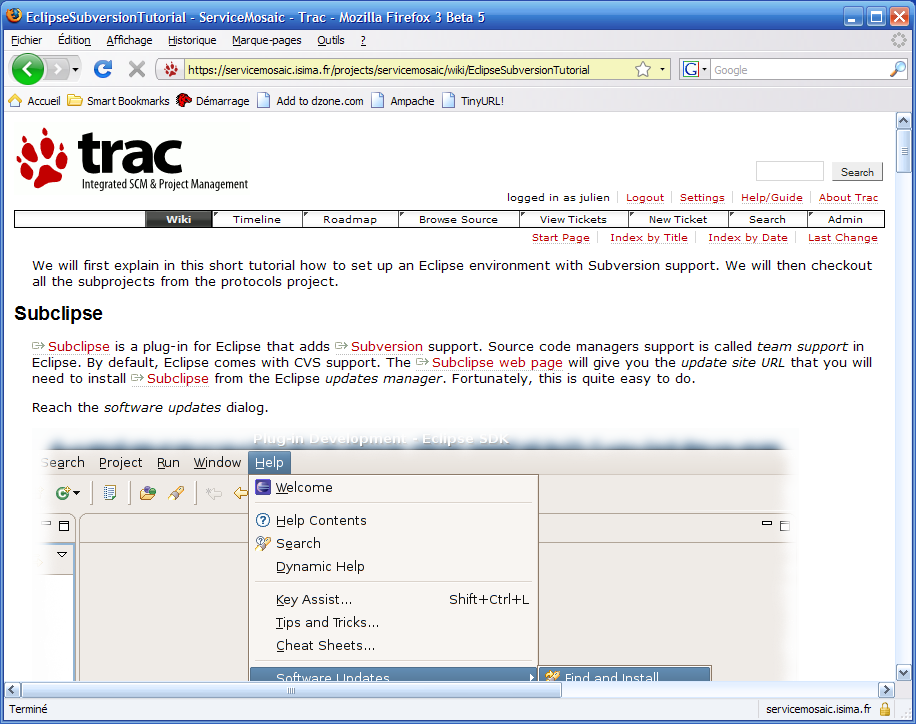
\includegraphics[width=\textwidth]{content/protocols-project/trac-wiki}
    \caption{Trac wiki view.}
    \label{fig:trac-wiki}
\end{figure}

\begin{figure}[tbhp]
    \centering
    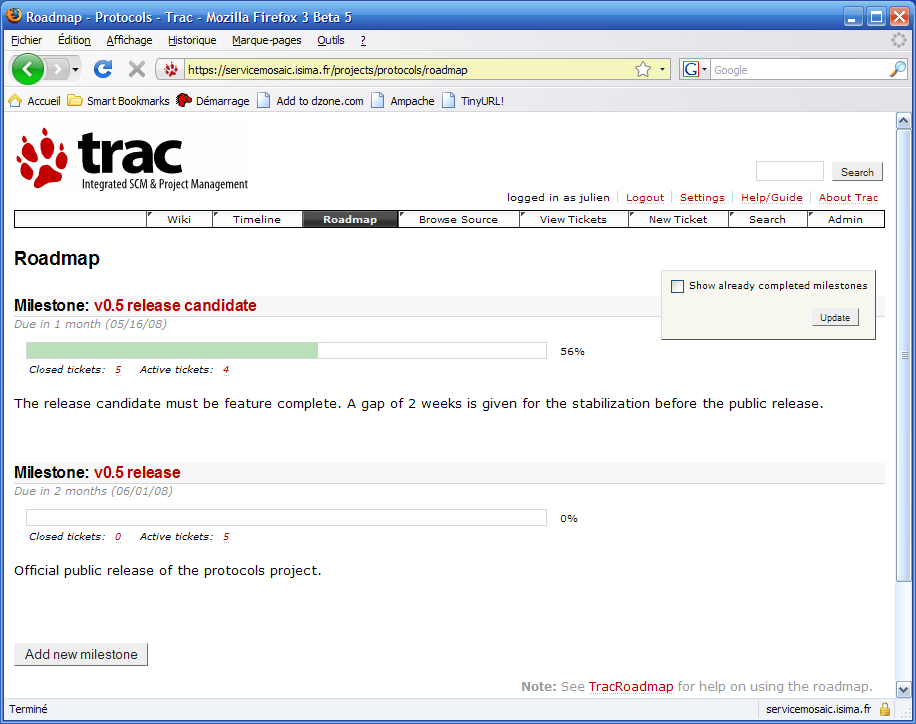
\includegraphics[width=\textwidth]{content/protocols-project/trac-roadmap}
    \caption{Trac roadmap view.}
    \label{fig:trac-roadmap}
\end{figure}

The platform being developed across different institutions around the world, we have deployed a server at \url{http://servicemosaic.isima.fr/} with collaborative services:
\begin{itemize}
  
  \item the source code management and versioning is done using Subversion (see \url{http://subversion.tigris.org/}), allowing for distributed, concurrent modifications and sharing of the source code bases
  
  \item each project has an instance of Trac (see \url{http://trac.edgewall.org/}), a web-based application for managing projects that offers a wiki (see Figure~\ref{fig:trac-wiki}), a source code browser (integrated with Subversion, see Figure~\ref{fig:trac-svn}), a roadmap (see Figure~\ref{fig:trac-roadmap}) and an issues manager (defects, tasks, enhancements, see Figure~\ref{fig:trac-issues}).
  
  \item mailing-lists and public / private download areas are available
  
  \item a JavaEE 5 compliant application server\footnote{In our case, we chose to run Glassfish from Sun Microsystems: \url{http://glassfish.org/}.} is available for the deployment of server-side applications, including web applications and web services.
  
\end{itemize}

\begin{figure}[tbhp]
    \centering
    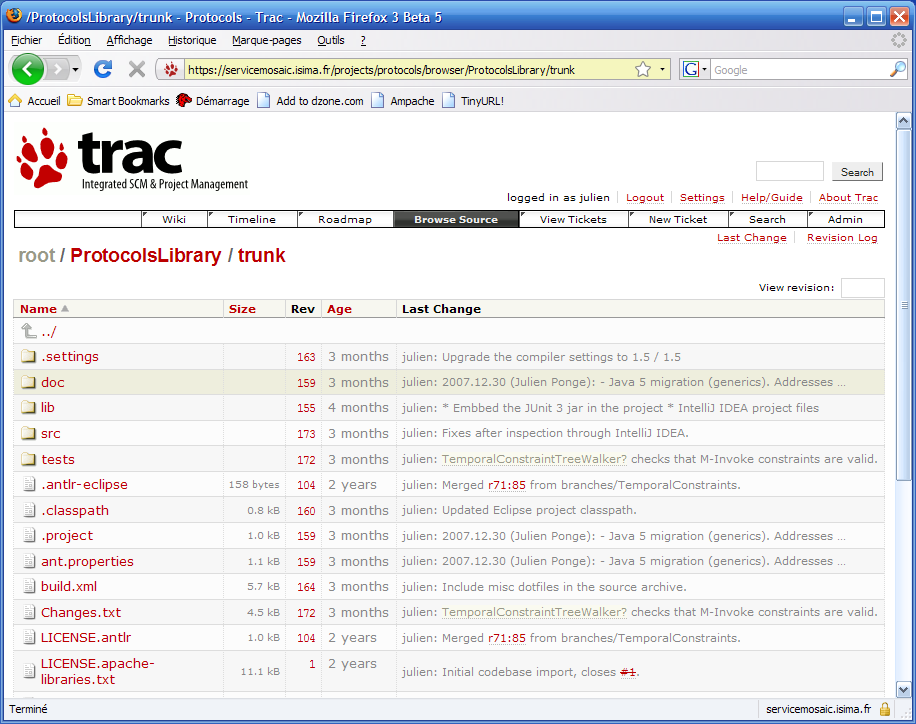
\includegraphics[width=\textwidth]{content/protocols-project/trac-svn}
    \caption{Trac source browser view.}
    \label{fig:trac-svn}
\end{figure}

\begin{figure}[tbhp]
    \centering
    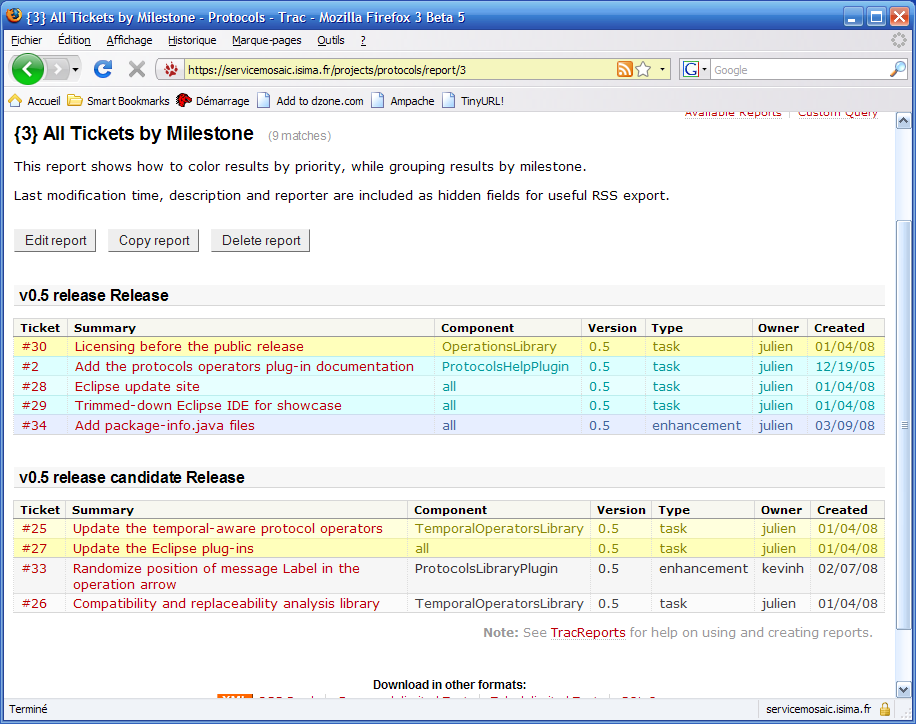
\includegraphics[width=\textwidth]{content/protocols-project/trac-issues}
    \caption{Trac issues management view.}
    \label{fig:trac-issues}
\end{figure}

A number of projects implemented as part of the ServiceMosaic platform are set to be progressively released to the public over time.

% ........................................................................... %

\section{Prototype: the ServiceMosaic Protocols project}

% ........................................................................... %

\begin{figure}[tbhp]
    \centering
    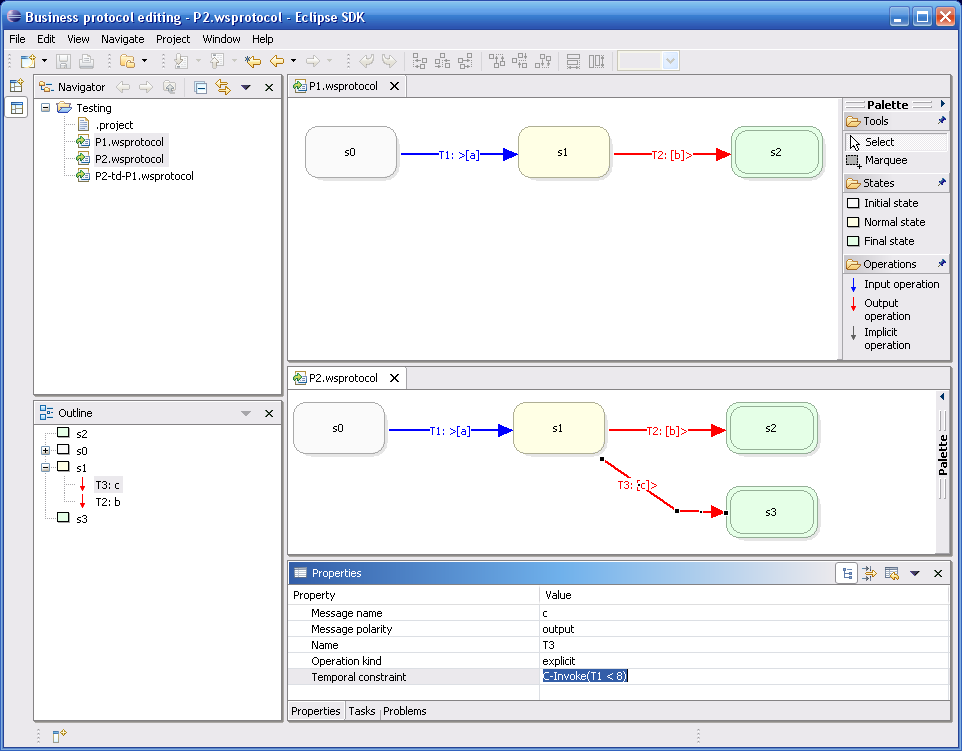
\includegraphics[width=\textwidth]{content/protocols-project/proto-screenshot}
    \caption{Screenshot of the ServiceMosaic Protocols prototype.}
    \label{fig:proto-screenshot}
\end{figure}

The work presented in this thesis has been implemented as part of a subproject of ServiceMosaic called \emph{ServiceMosaic Protocols}. It groups the libraries and development tools that are related to business protocol modeling, analysis and management. Figure~\ref{fig:proto-screenshot} shows a screenshot of the prototype development environment which is based on the Eclipse platform. It features two business protocol being edited, including timing constraints.

% ........................................................................... %

\subsection{Components}

% ........................................................................... %

\begin{figure}[tbhp]
    \centering
    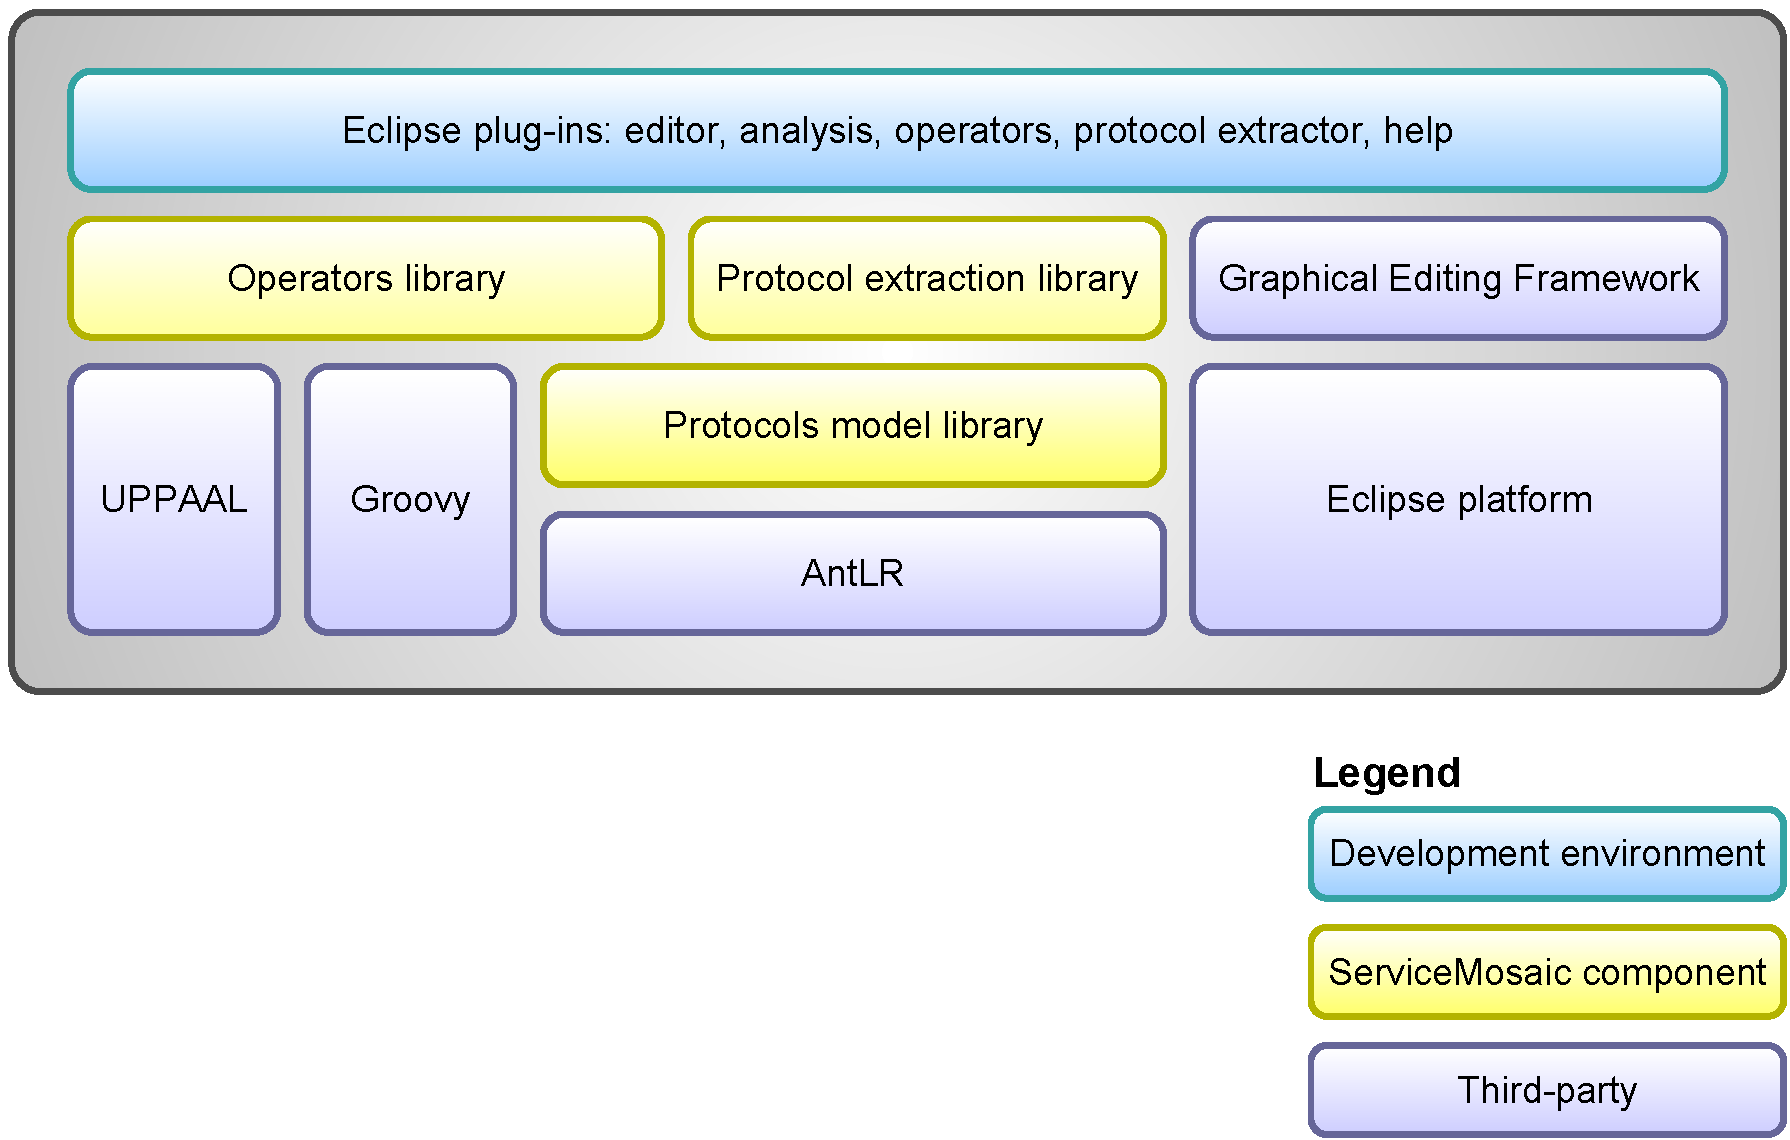
\includegraphics[width=\textwidth]{content/protocols-project/protocols-proto-layers}
    \caption{Architecture of the ServiceMosaic Protocols prototype.}
    \label{fig:protocols-proto-layers}
\end{figure}

The following components have been developed as part of the ServiceMosaic Protocols project, as depicted on Figure~\ref{fig:protocols-proto-layers}.
\begin{description}
  
  \item[A business protocols model library] has been developed. It contains an object-oriented model for representing and manipulating business protocols. While abstracting from the physical representation of protocols (e.g, files, databases, ...), it contains a simple XML persistence class that allows protocols to be stored and read from various XML sources (e.g., files, XML databases, network interface, ...). Temporal constraints are explicitly supported by the library. They are stored as plain strings in the model that are attached to the transitions of a protocol. However, a complete object model is part of the library for manipulating temporal constraints (e.g., programmatically constructing an in-memory constraint, computing the conjunction of two constraints, renaming variables, computing the negation of a constraint, ...). We use a parser written using AntLR\footnote{AntLR is actively developed at \url{http://www.antlr.org/}.} \cite{ParrQ95} for obtaining the object model that corresponds to a constraint in a plain string and vice-versa. As such, the protocol model library is self-contained.
  
  \item[A protocol manipulation and comparison operators library] has been developed using the Groovy language  \cite{Groovy07}. It implements the complete range of business protocol operators (i.e., $\intersop$, $\compop$, $\diffop$, $\sqsubseteq$, $\equiv$). The operators can be used ``as-is'', or a facade class can be used for directly assessing compatibility or replaceability between two protocols. In fact, the facade class does nothing but invokes the manipulation and comparison operators as described in Table~\ref{tab:classes-characterization}. Emptiness checking is required by some operators. It is done using the UPPAAL model checker using the technique that is presented from page~\pageref{chap:uppaal-pta}.
  
  \item[A set of Eclipse plug-ins] have been developed, based on the libraries mentioned above and the Eclipse platform. The business protocol editor is based on a set of customized SWT/JFace figures (e.g., the shape of states in a protocol) and the Eclipse Graphical Editing Framework (see \url{http://www.eclipse.org/gef/}). It can take advantage of WSDL documents for ensuring that only valid messages are being put into protocols by designers. The analysis components provide a visual interface for either invoking the manipulation and comparison operators, or directly checking for compatibility and replaceabilty of protocols. An embedded help support is available for providing assistance.
  
\end{description}

The figure also depicts a \emph{protocol extraction} component. This companion component having been developed by an engineering intern of the APIS Research Group\footnote{See \url{http://apis.isima.fr/}.}, and since it is still very experimental at this stage, it will be presented separately in the following section.\\

To make the libraries easier to use, we adopted the use of \emph{fluent interfaces} \cite{FowlerFI05}. Briefly, such ``fluent'' interfaces tend to use techniques such as making method calls chainable. This arguably makes the code sometimes easier to read, and in many cases, fluent interfaces can be enough for making an \emph{internal domain-specific language} \cite{FreemanP06,FowlerDSL04}. \\

The components developed in this project have served as the basis of many other ServiceMosaic projects. For example, the protocols model library serves as the standard ServiceMosaic library for developing components that manipulate protocols. Also, the protocol editor has been used in derivative works such as the protocol discovery and refinement tool \cite{Motahari-NezhadSBC07}.\\

The ServiceMosaic Protocols project are staged to be released in 2008 under the terms of the \emph{GNU Lesser General Public License version 3}\footnote{See \url{http://www.gnu.org/licenses/lgpl.html}.}, a moderate open-source license that facilitates dissemination of the work while enforcing modifications of the code to be released under the same licensing conditions.

% ........................................................................... %

\subsection{Protocol extraction}

% ........................................................................... %

We now outline a \emph{protocol extraction operator}, developed externally as part of the ServiceMosaic project, that takes a BPEL process as input and outputs a \emph{multi-party protocol}, which is basically an extension of a timed protocol where a message is also tagged with the \emph{partner link} of the service which is sending or receiving the message.
Hence, a multi-party business protocol captures the global message \emph{choreography} of a BPEL process.\\

To extract the multi-party protocol we proceed as follows.
First, we identify \emph{protocol extraction patterns} for each type of  basic and complex BPEL activity. The extraction starts from the beginning of the process and goes through each activity to apply the protocol extraction patterns as such they are recognized. When a complex activity is encountered (e.g., \emph{if}, \emph{switch}, \emph{while}, \emph{pick}, ...), it is recursively processed on each of its complex activities until basic activities are reached. Hence, the obtained protocol fragments are assembled by inverse recursion. For instance, if a \emph{if} activity comprises one \emph{invoke} on each alternative branch, then a protocol fragment is derived from each \emph{invoke}, then they are combined as different branches from the current state in the extraction process.\\

\begin{figure}[tbhp]
    \centering
    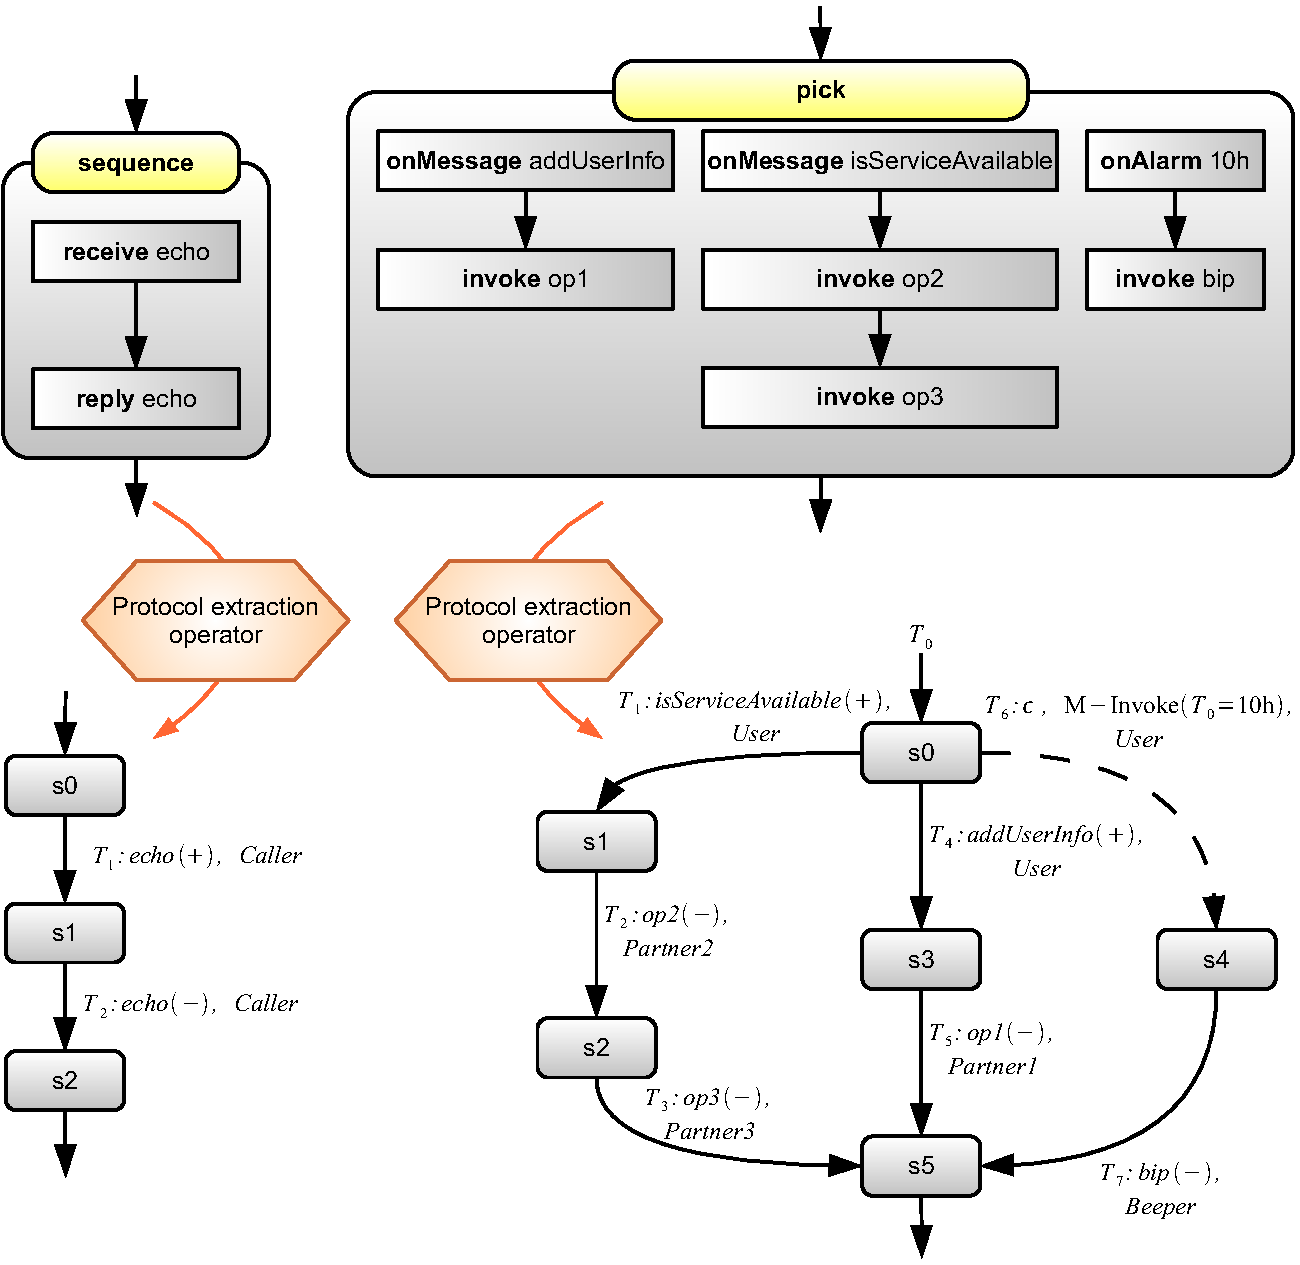
\includegraphics[width=\textwidth]{content/protocols-project/bpel2protocol}
    \caption{Extraction of multi-party protocols fragments from BPEL.}
    \label{fig:bpel2protocol}
\end{figure}

We give two examples of BPEL patterns extractions on Figure~\ref{fig:bpel2protocol}. The first example shows a simple \emph{sequence} activity that consists of a \emph{receive} activity followed by a \emph{reply}. What is done by the sequence is simply the echo-ing of a message. This is translated using two transitions (one for each message). Because a multi-party protocol is extracted, each transition is also tagged with the partner link (e.g. \emph{Caller}) and the BPEL activity (e.g. \emph{reply}).\\

The second example shows a \emph{pick} complex activity involving two message handlers and an alarm handler. Each message or alarm handler leads to a branch for the message choreography that corresponds to its activities. For example on the \emph{addUserInfo} message handler, there is a $op1$ invocation on the \emph{Partner1} partner link. The \emph{onAlarm} handler leads to an implicit transition featuring a \MInvoke constraint. Temporal informations can be extracted from either \emph{onAlarm} handlers or \emph{wait} activities. Finally, all branches join in the state $s_5$ which corresponds to the end of the \emph{pick} activity.\\

Note that this transformation is not reversible. When generating a protocol, we only care about possible ordering of messages and not about the many details prescribed by a BPEL process (such as why -- based on which condition -- a certain path is chosen). Nevertheless, we had developed developed techniques for generating service implementation templates in BPEL from protocols definitions \cite{KBBB+04}.\\

The protocol which is followed by the process while interacting with a given service (identified by its BPEL \emph{partner link}) can be obtained as follows. The idea is to perform a special form of filtering on the multi-party protocol. In a similar fashion as \emph{projection} for timed automata \cite{RAPM04}, we replace the messages with $\varepsilon$ on the transitions that are not associated with the partner link of the service that we are interested in. Also, each temporal constraint that refers to a transition which is not from the target partner link is removed. Indeed, they do not make sense in the protocol that we want to obtain since they refer to events that are not ``seen'' by the orchestrated service. Finally, the service protocol is obtained by removing the $\varepsilon$ transitions using standard techniques on automata \cite{Hopcroft79}. This is possible only because if we mapped to timed automata, there would be no guard nor clock resets on these transitions \cite{VDPG97}.\\

In our experiments, we have found out that the protocol extraction operator works well for a large majority of BPEL processes. As mentioned previously, this protocol extraction operator is absolutely not part of this thesis work contributions. It will require further investigations, including formalization, a proper theoretical study and implementation work.

% ........................................................................... %
